\documentclass[aspectratio=169,11pt]{beamer}
\usepackage[T1]{fontenc}
\usepackage{lmodern,amsmath,amssymb,mathtools,bm,booktabs,array,graphicx,tikz}
\usetikzlibrary{arrows.meta,positioning,calc,decorations.pathreplacing,patterns}
\definecolor{ink}{HTML}{17344D}\definecolor{accent}{HTML}{087E8B}\definecolor{pale}{HTML}{EDF5F5}\definecolor{gold}{HTML}{AD6B19}
\providecommand{\dd}{\,\mathrm{d}}\providecommand{\R}{\mathbb{R}}
\providecommand{\E}{\mathbb{E}}\providecommand{\Var}{\operatorname{Var}}
\providecommand{\Cov}{\operatorname{Cov}}\providecommand{\diag}{\operatorname{diag}}
\providecommand{\norm}[1]{\left\lVert#1\right\rVert}
\providecommand{\abs}[1]{\left|#1\right|}
\usefonttheme{professionalfonts}
\setbeamercolor{normal text}{fg=black,bg=white}
\setbeamercolor{frametitle}{fg=ink,bg=white}
\setbeamercolor{title}{fg=ink}\setbeamercolor{structure}{fg=accent}
\setbeamercolor{block title}{fg=ink,bg=pale}\setbeamercolor{block body}{fg=black,bg=pale!40}
\setbeamercolor{alerted text}{fg=accent}
\setbeamerfont{frametitle}{size=\Large,series=\bfseries}
\setbeamerfont{title}{size=\LARGE,series=\bfseries}
\setbeamertemplate{navigation symbols}{}
\setbeamersize{text margin left=.7cm,text margin right=.7cm}
\setbeamertemplate{frametitle}{\vspace{.18cm}\insertframetitle\par\vspace{.1cm}{\color{accent}\hrule height .6pt}\vspace{.12cm}}
\newcommand{\notestarget}{notes.pdf}\newcommand{\noteslabel}{Notes}
\setbeamertemplate{footline}{\hspace{.7cm}\color{ink}\scriptsize Scientific Computing in Python\quad\href{\notestarget}{\noteslabel}\hfill\insertframenumber\,/\,\inserttotalframenumber\hspace{.7cm}\vspace{.18cm}}
\setbeamercovered{invisible}
\hypersetup{pdfauthor={Zan Ahmad},pdftitle={ODE integration, root finding, and parameter estimation},pdfpagemode=UseNone}
\begin{document}
\begin{frame}[plain]\vfill
{\small\color{accent} Scientific Computing in Python \quad Lecture 4}\par\medskip
{\raggedright\hyphenpenalty=10000\exhyphenpenalty=10000\LARGE\bfseries\color{ink} ODE integration, root finding, and parameter estimation}\par\bigskip
Zan Ahmad\par\smallskip
{\small Winter 2026}\par\vfill\end{frame}
\renewcommand{\notestarget}{notes.pdf\#note-newton-s-cooling-equation}
\begin{frame}[t,fragile,label=slide-newton-s-cooling-equation]{Newton's cooling equation}
\[
\dot T=-k(T-T_a),\qquad T(0)=T_0.
\]
\pause{}
Set $u=T-T_a$. Then $\dot u=-ku$, and $k$ has units of inverse time.
\end{frame}
\renewcommand{\notestarget}{notes.pdf\#note-newton-s-cooling-equation}
\begin{frame}[t,fragile,label=slide-exact-solution]{Exact solution}
\[
\frac{\dd u}{u}=-k\,\dd t
\quad\Longrightarrow\quad
\log\left|\frac{u(t)}{u(0)}\right|=-kt.
\]
\pause{}
\[
T(t)=T_a+(T_0-T_a)e^{-kt}.
\] For $u(0)=0$, use the constant solution $u(t)=0$.
\end{frame}
\renewcommand{\notestarget}{notes.pdf\#note-time-scales-and-forward-euler}
\begin{frame}[t,fragile,label=slide-time-scales-and-forward-euler]{Time scales and forward Euler}
\[
T_{n+1}=T_n-hk(T_n-T_a),\qquad
u_{n+1}=(1-kh)u_n.
\]
\pause{}
Decay requires $|1-kh|<1$, or $0<kh<2$.
\end{frame}
\renewcommand{\notestarget}{notes.pdf\#note-time-scales-and-forward-euler}
\begin{frame}[t,fragile,label=slide-monotone-versus-oscillatory-decay]{Monotone versus oscillatory decay}
\[
0<kh\leq1:\quad u_n\text{ preserves sign and decays},
\]
\pause{}
\[
1<kh<2:\quad u_n\text{ alternates sign while decaying}.
\]
The second behavior is numerically stable but inconsistent with monotone cooling in this model.
\end{frame}
\renewcommand{\notestarget}{notes.pdf\#note-adaptive-integration}
\begin{frame}[t,fragile,label=slide-adaptive-integration]{Adaptive integration}
\begin{verbatim}
sol = solve_ivp(rhs, (0, 8), [80],
                t_eval=times, rtol=1e-8, atol=1e-10)
\end{verbatim}
\pause{}
Compare $T_{\rm num}(t_i)$ with $20+60e^{-0.4t_i}$.
\end{frame}
\renewcommand{\notestarget}{notes.pdf\#note-linear-interpolation}
\begin{frame}[label=slide-cooling-trajectory-and-interpolation-error-figure]{Cooling trajectory and interpolation error}
\centering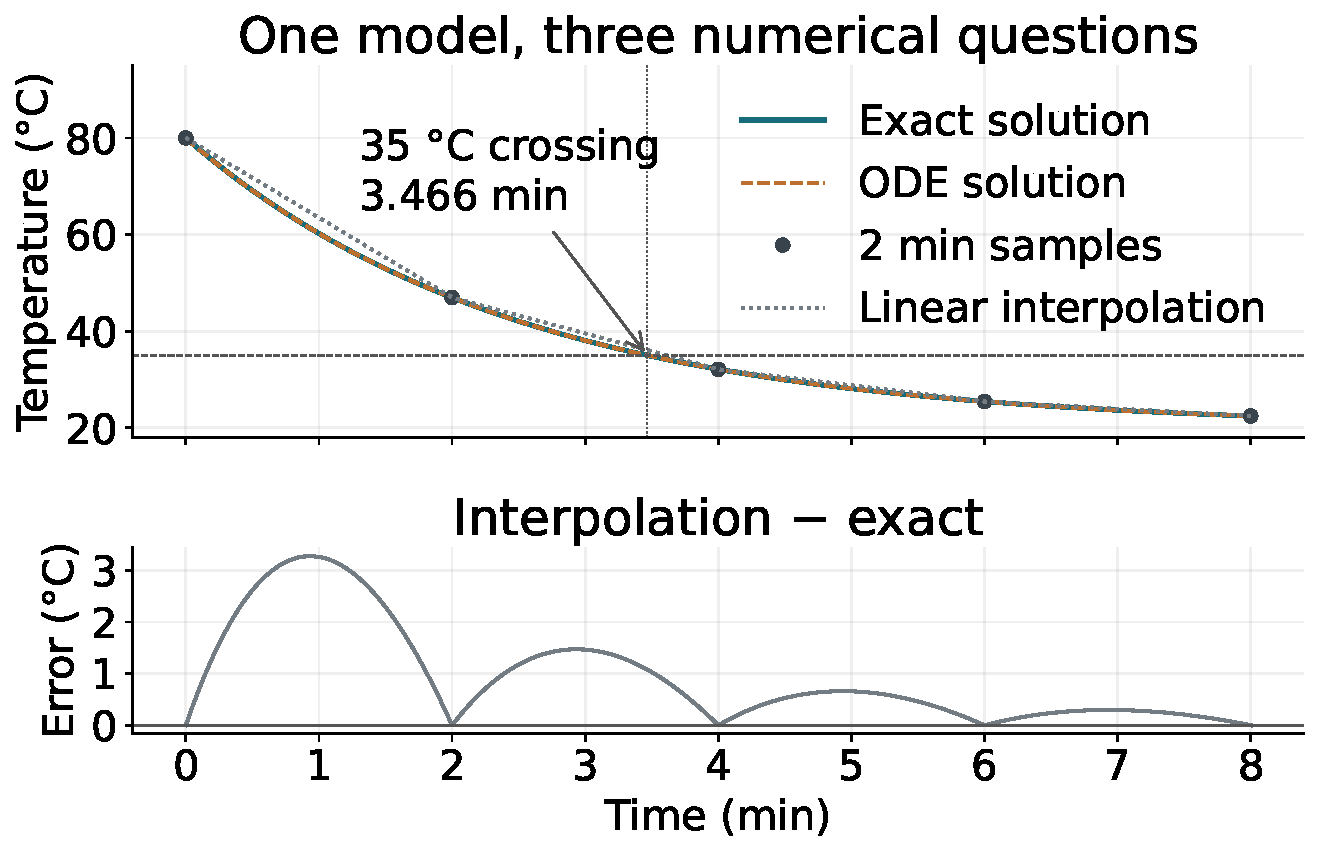
\includegraphics[width=.98\linewidth,height=.69\textheight,keepaspectratio]{cooling-questions.pdf}\end{frame}
\renewcommand{\notestarget}{notes.pdf\#note-linear-interpolation}
\begin{frame}[t,fragile,label=slide-error-under-refinement]{Error under refinement}
\[
E(h)=\max_i|T_h(t_i)-T(t_i)|.
\]
\pause{}
For first-order Euler convergence, $E(h)/E(h/2)$ approaches $2$ when the step is sufficiently small and roundoff does not dominate.
\end{frame}
\renewcommand{\notestarget}{notes.pdf\#note-threshold-time-as-a-root}
\begin{frame}[t,fragile,label=slide-threshold-time-as-a-root]{Threshold time as a root}
\[
T_*-T_a=(T_0-T_a)e^{-kt_*}.
\]
\pause{}
\[
t_* =\frac1k\log\frac{T_0-T_a}{T_*-T_a}.
\]
\end{frame}
\renewcommand{\notestarget}{notes.pdf\#note-threshold-time-as-a-root}
\begin{frame}[t,fragile,label=slide-a-threshold-calculation]{A threshold calculation}
For $T_0=80$, $T_a=20$, $k=0.4$ and $T_*=40$,
\[
t_* =2.5\log3\approx2.74653\ \mathrm{min}.
\]
\pause{}
The logarithm's argument is dimensionless and greater than one.
\end{frame}
\renewcommand{\notestarget}{notes.pdf\#note-linear-interpolation}
\begin{frame}[t,fragile,label=slide-linear-interpolation]{Linear interpolation}
\[
\widetilde T(t)=(1-\alpha)T_i+\alpha T_{i+1},\qquad
\alpha=\frac{t-t_i}{t_{i+1}-t_i}.
\]
\pause{}
Here $0\leq\alpha\leq1$ only within the sampled interval.
\end{frame}
\renewcommand{\notestarget}{notes.pdf\#note-fitting-the-cooling-coefficient}
\begin{frame}[label=slide-parameter-objective-and-residuals-figure]{Parameter objective and residuals}
\centering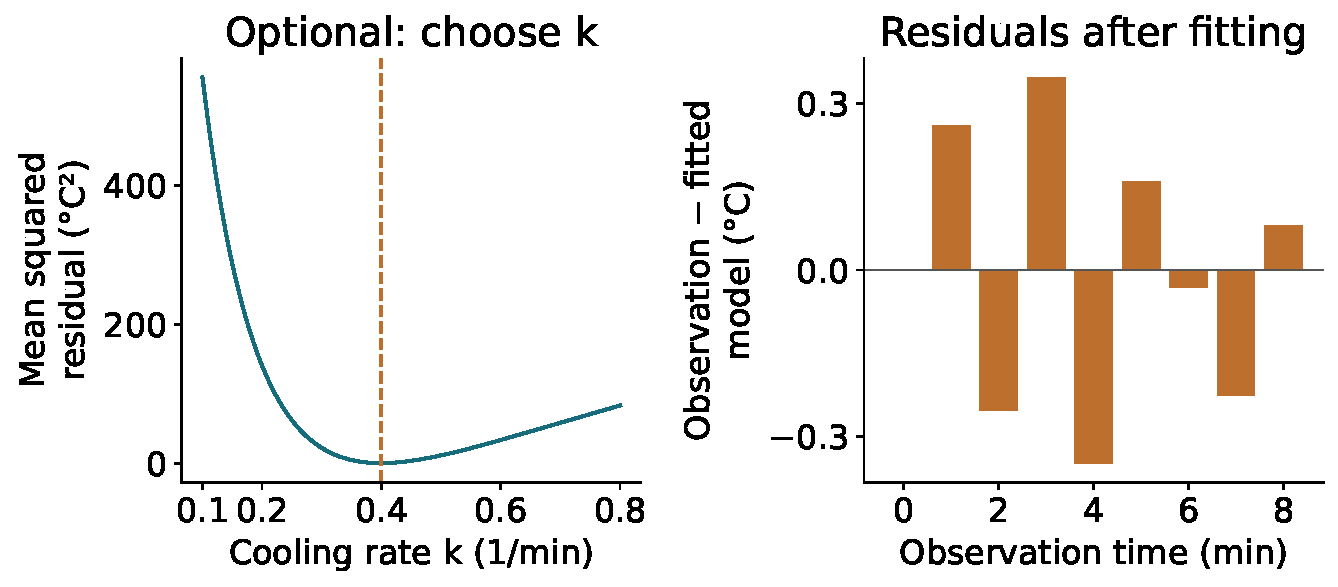
\includegraphics[width=.98\linewidth,height=.69\textheight,keepaspectratio]{fit-and-residuals.pdf}\end{frame}
\renewcommand{\notestarget}{notes.pdf\#note-linear-interpolation}
\begin{frame}[t,fragile,label=slide-interpolation-error-for-cooling]{Interpolation error for cooling}
\[
T(t)-\widetilde T(t)=\frac{T''(\xi)}2(t-t_i)(t-t_{i+1}).
\]
\pause{}
Cooling from above ambient has $T''>0$. The product is nonpositive inside the interval, so the secant lies above the exact curve.
\end{frame}
\renewcommand{\notestarget}{notes.pdf\#note-fitting-the-cooling-coefficient}
\begin{frame}[t,fragile,label=slide-fitting-the-cooling-coefficient]{Fitting the cooling coefficient}
\[
J(k)=\frac1n\sum_i[T_a+(T_0-T_a)e^{-kt_i}-y_i]^2.
\]
\pause{}
\[
\frac{\partial T(t;k)}{\partial k}=-t(T_0-T_a)e^{-kt}.
\]
\end{frame}
\renewcommand{\notestarget}{notes.pdf\#note-fitting-the-cooling-coefficient}
\begin{frame}[t,fragile,label=slide-sensitivity-in-time]{Sensitivity in time}
At $t=0$, the temperature is independent of $k$. At very long times it is nearly ambient and again weakly sensitive.
\pause{}
For $t>0$, the magnitude $te^{-kt}$ is largest at $t=1/k$. Measurements near that scale are informative about $k$.
\end{frame}
\end{document}
